\documentclass[12pt]{article}

\usepackage{sbc-template}

\usepackage{graphicx,url}

\usepackage[brazil]{babel}   
%\usepackage[latin1]{inputenc}  
\usepackage[utf8]{inputenc}  
% UTF-8 encoding is recommended by ShareLaTex

\usepackage{tikz}
\usetikzlibrary{shapes,snakes}

\definecolor{myblack}{cmyk}{0.94,0.54,0,0}

\tikzstyle{snippet}=[draw=myblue,fill=none,thick,
                   text width=0.85\textwidth,rectangle,
                   rounded corners=0pt,inner sep=0pt,inner ysep=10pt]
\tikzstyle{title}=[fill=white,text=myblue,rectangle]
     
\sloppy

\title{Relatório sobre Implementação NAT e RIP}

\author{Edgar Santos\inst{1} Leonardo Gubert\inst{1}, Matheus Redecker\inst{1}}


\address{Pontifícia Universidade Católica do Rio Grande do Sul - PUCRS
  \email{  \{edgar.sdsantos@gmail.com\} 
  \{leonardo.gubert, matheus.redecker\}{@acad.pucrs.br} }
}

\begin{document} 

\maketitle

Neste artigo é demonstrado a implementação de uma rede virtual (Vlan) com protocolo de roteamento RIP e uma configuração de NAT num roteador CISCO. Para implementação da rede, foi utilizado o terminal do modem baseado em texto, chamado MINICOM.

Temos como a topologia proposta a seguir:

\begin{figure}[h]
\centering
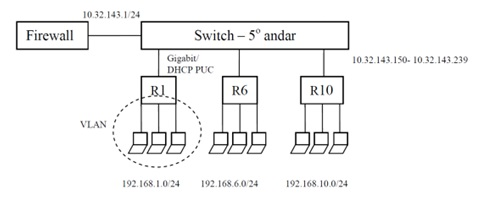
\includegraphics[scale=1]{topologia.jpg}
\caption{Topologia da Rede}
\label{topologia}
\end{figure}

Tomaremos como base o roteador R1, como descrito na Figura \ref{topologia} para criarmos nossa rede privada. 
Para criação da Vlan, é necessário mapear a interface Gigabit no computador 1 para que seja criado uma Vlan. Dada a subrede 192.168.1.0/24 do roteador, optamos por designar o IP 192.168.1.1/24 para que seja o IP da nossa rede privada, assim como o DNS padrão para 8.8.8.8. Segundo passo é criar uma rota entre a nossa subrede e a interface Gigabit.No ambiente disponibilizado no laboratório, existem baias nas quais 3 computadores estão conectados num mesmo cabeamento que pertencente a rede do roteador CISCO que estamos configurando, devemos desabilitar a interface Gigabit e disponibilizar apenas a conexão a Vlan criada. Seguido estes passos, para que o segundo computador seja conectado à rede Vlan, devemos habilitar o DHCP na rede Vlan no terminal Minicom para que um IP seja fornecido ao computador 2. Assim, temos uma rede Vlan de para cada computador ligado ao roteador que configuramos, mas essas Vlans não consegue enviar ou receber dados da internet. Para que a Vlan tenha conexão a rede externa, devemos fazer algumas configurações. Atualmente, a subrede do R1, não faz o roteamento ou muito menos tem conhecimento da Vlan, para isto devemos configurar no Minicom do computador 1 a habilitação do protocolo de roteamento RIP na porta de roteamento do R1. Para que exista comunicação entre a Vlan e a rede externa, também devemos configurar o NAT. A primeira etapa na implantação do NAT é definir o as interfaces internas e externas, ou seja, para que os usuários da Vlan se conectem a internet, devemos autorizar certos dispositivos internos a iniciar comunicação com os dispositivos externos convertendo seus endereços inválidos em um endereço ou um pool de endereços válidos.
Para isso acontecer devemos efetuar os seguintes passos no terminal minicom e então conseguimos comunicação com a rede Internet.

\begin{tikzpicture}
  \node[snippet](box){
interface serial 0 \\ 
ip address 10.32.143.1 255.255.255.0 \\
ip nat outside \\
- \\
interface eth0 \\
ip address 192.168.1.0 255.255.255.0 \\
ip nat inside \\
- \\
ip nat pool no-overload 10.32.143.1 prefix 24 \\
- \\
ip nat inside source list 7 pool no-overload \\
- \\
access-list 7 permit10.32.143.1  0.0.0.24 \\
};;
\node[title] at (box.north) {};
\end{tikzpicture}


\end{document}
